%%%%%%%%%%%%%%%%%%%%%%
% Wenneker Resume/CV %
%%%%%%%%%%%%%%%%%%%%%%
\documentclass[a4paper,12pt]{memoir} % Font and paper size

\usepackage{multirow}
\input{structure.tex} % Include the file specifying document layout and packages

%----------------------------------------------------------------------------------------
%	NAME AND CONTACT INFORMATION 
%----------------------------------------------------------------------------------------

\userinformation{ % Set the content that goes into the sidebar of each page
\begin{flushright}
% Comment out this figure block if you don't want a photo
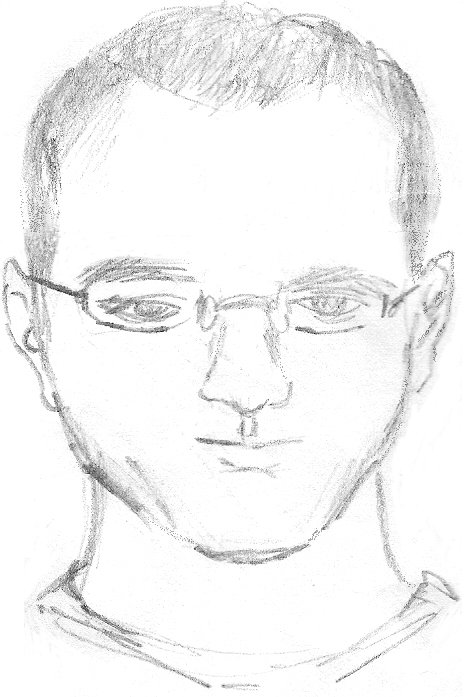
\includegraphics[width=\columnwidth]{lex.png}\\[\baselineskip] % Your photo
\large \textbf{Alex Towell} \\
\small \href{mailto:lex@metafunctor.com}{lex@metafunctor.com} \\
\vspace{0.5cm}
\href{https://metafunctor.com}{metafunctor.com} \\
\href{https://github.com/queelius}{github.com/queelius} \\
\vspace{0.5cm}
(618) 977-1746 \\ % Your phone number
\vfill % Whitespace under this block to push it up under the photo
\end{flushright}
}

%----------------------------------------------------------------------------------------

\begin{document}

\userinformation % Print your information in the left column

\framebreak % End of the first column

%----------------------------------------------------------------------------------------
%	HEADING
%----------------------------------------------------------------------------------------

\cvheading{Alex Towell} % Large heading - your name

\cvsubheading{PhD Student | AI/ML Research | Mathematics}

%-------------------------------------------------------------------------
%----------------------------------------------------------------------------------------
%	ABOUT ME
%----------------------------------------------------------------------------------------

\aboutme{About Me}{PhD student in Computer Science focused on reliable and secure ML systems. My current work studies adversarial robustness in ransomware prevention; in controlled experiments our approach achieved a $10^{-8}$ false-negative rate. I prefer careful, incremental engineering, clear writing, and reproducible results. I build data and backend systems, contribute to open-source tools, and am especially interested in AI safety, evaluation, and interpretability.}

%----------------------------------------------------------------------------------------
%	EDUCATION
%----------------------------------------------------------------------------------------

\CVSection{Education}

\CVItem{2024 - Present, Southern Illinois University}{PhD in Computer Science}
{
    \begin{itemize}
        \item Research Focus: AI Safety, Alignment, Mechanistic Interpretability, Adversarial Robustness
        \item Advisor: Dr. Hiroshi Fujinoki
        \item Expected Graduation: 2028
    \end{itemize}
}

\Sep

%------------------------------------------------

\CVItem{2021 - 2023, Southern Illinois University-Edwardsville}{MS in Mathematics}
{
    \begin{itemize}
        \item GPA: 3.9/4.0
        \item Concentration: Statistics and Operations Research
        \item Awarded R.N. Pendergrass Graduate Scholarship
    \end{itemize}
}

\Sep

%------------------------------------------------

\CVItem{2012 - 2015, Southern Illinois University-Edwardsville}{MS in Computer Science}
{
    \begin{itemize}
        \item GPA: 4.0/4.0
        \item Concentration: Artificial Intelligence
        \item Awarded Outstanding Graduate Student (School of Engineering)
    \end{itemize}
}

\Sep

%------------------------------------------------

\CVItem{2006 - 2010, Southern Illinois University-Edwardsville}{BS in Computer Science}
{
    \begin{itemize}
        \item GPA: 3.6/4.0
        \item Awarded Outstanding Junior (Dept. of Computer Science)
    \end{itemize}
}

%------------------------------------------------

\Sep

%----------------------------------------------------------------------------------------
% TECHNICAL SKILLS
%----------------------------------------------------------------------------------------

\CVSection{Technical Skills}

\CVItem{Languages}{Python (primary), R, C/C++, Java, TypeScript, Bash, LaTeX}\\
\CVItem{AI/ML}{PyTorch, HuggingFace Transformers, CUDA, LLM fine-tuning, NumPy, Pandas}\\
\CVItem{Systems}{Linux, Docker, Git, PostgreSQL, Elasticsearch, Redis, REST APIs}\\
\CVItem{Open Source}{Contributor/maintainer; code review; documentation; small tooling}\\

\clearpage % Start a new page

\userinformation % Print your information in the left column

\framebreak % End of the first column

%----------------------------------------------------------------------------------------
%	PUBLICATIONS
%----------------------------------------------------------------------------------------

\CVSection{Publications}

\begin{itemize}
    \item H. Fujinoki, \textbf{A. Towell}, V.A. Thota, ``Preventing Ransomware Damages using In-Operation Off-Site Backup to Achieve a $10^{-8}$ False-Negative Miss-Detection Rate,'' \textit{International Conference on Computing and Intelligence (ICCI)}, 2025
    \item \textbf{A. Towell}, ``Reliability Estimation in Series Systems: Maximum Likelihood Techniques for Right-Censored and Masked Failure Data,'' Master's Project, Department of Mathematics and Statistics, Southern Illinois University Edwardsville, 2023
    \item \textbf{A. Towell}, H. Fujinoki, ``Estimating How Confidential Encrypted Searches Are Using Moving Average Bootstrap Method,'' \textit{IEEE International Conference on Cloud Computing Technology and Science (CloudCom)}, 2016
    \item \textbf{A. Towell}, ``Encrypted Search: Enabling Standard Information Retrieval Techniques Using New Secure Index Types,'' Master's Thesis, ProQuest Dissertations \& Theses, 2015
\end{itemize}

\Sep

%----------------------------------------------------------------------------------------
% SELECTED RESEARCH AND PROJECTS
%----------------------------------------------------------------------------------------

\CVSection{Selected Research \& Projects}

\CVItem{AlgoTree}{Python utilities for tree-like data (FlatForest/TreeNode) with a CLI (\texttt{jt}) to query and manipulate hierarchical data; used for inspecting nested structures.}\\
\CVItem{Elasticsearch-LM}{Prototype fine-tuning to translate natural language into Elasticsearch Query DSL using transformers and synthetic data; evaluates translation accuracy and failure modes.}\\
\CVItem{Reverse-Process Synthetic Data}{Exploratory algorithms to generate math-reasoning training data; emphasis on data quality, clear assumptions, and reproducibility.}\\
\CVItem{Oblivious Computation}{Explored space–security trade-offs for privacy-preserving computation; built small prototypes for workload partitioning.}\\
\CVItem{IDOT D8 Infrastructure System}{Lead developer for a traffic-monitoring system; proposed and planning multimodal models to assess incidents and camera quality. Designed for reliability, auditability, and straightforward operations.}

\clearpage % Start a new page

\userinformation % Print your information in the left column

\framebreak % End of the first column

%----------------------------------------------------------------------------------------
% ACADEMIC EXPERIENCE
%----------------------------------------------------------------------------------------

\CVSection{Academic Experience}

\CVItem{2024--Present, Research Assistant, SIU}{
    \begin{itemize}
        \item Cybersecurity research with Dr. Hiroshi Fujinoki on ransomware detection using probabilistic data structures and careful evaluation
        \item Built prototypes for telemetry analysis and automated response with LLMs; documented limits and failure cases
        \item Lead developer for Illinois Department of Transportation District 8 (IDOT D8) application with planned multimodal AI components
        \item Co-authored study reporting $10^{-8}$ false-negative miss-detection under controlled conditions (ICCI 2025)
    \end{itemize}
}

\Sep

\CVItem{2021--2022, Teaching Assistant, SIUE}{
    \begin{itemize}
        \item Taught lab courses in mathematics and statistics
    \end{itemize}
}

\Sep

\CVItem{2012--2015, Research/Graduate/Teaching Assistant, SIUE}{
    \begin{itemize}
        \item Supported research in AI and machine learning while pursuing MS in Computer Science
        \item Taught undergraduate computer science lab sessions
        \item Developed encrypted search algorithms for confidential data retrieval systems
    \end{itemize}
}

\end{document}
